%==============================================================================
% Verdedigingsslides bachelorproef
% De effectiviteit van gamification bij het aanleren van COBOL aan junior
% developers (Learn COBOL)
%==============================================================================
% Compileer met XeLaTeX. Bv.:
%   latexmk -xelatex presentatie.tex
% Bronverwijzingen via biblatex/biber, hergebruik van bachproef.bib.
% Stijl: https://github.com/HoGentTIN/latex-hogent-beamer

\documentclass[aspectratio=169,11pt]{beamer}

%==============================================================================
% Aanloop
%==============================================================================

\usetheme{hogent}
\usecolortheme{hgwhite}

% Reserveer ruimte voor paginanummer en HOGENT-logo in de footer
\setbeamersize{text margin right=3.4cm}
\setbeamercolor{page number in foot}{fg=black}
\setbeamerfont{page number in foot}{size=\scriptsize}
\setbeamertemplate{footline}{%
  \begin{beamercolorbox}[wd=\paperwidth,ht=1cm,dp=0.9cm,leftskip=1em]{footline}
    \usebeamercolor[fg]{page number in foot}%
    \usebeamerfont{page number in foot}%
    \insertframenumber/\inserttotalframenumber
    \hfill
    \begin{tikzpicture}[remember picture, overlay]
      \node [anchor=south east, shift={(-\the\wd\logopart, \the\wd\logopart)},
      inner sep=0, outer sep=0] at (current page.south east)%
      {%
        
\includegraphics[height=\the\ht\logopart]{hogent_logo}%
      };%
    \end{tikzpicture}
  \end{beamercolorbox}
}

\setbeamerfont{frametitle}{series=\bfseries,size=\Large}
\setbeamertemplate{frametitle}{%
  \nointerlineskip
  \vskip0.75ex
  \begin{beamercolorbox}[wd=\paperwidth,leftskip=1em,rightskip=1em,dp=1.2ex]{frametitle}
    \usebeamerfont{frametitle}\strut\insertframetitle\strut\par
  \end{beamercolorbox}%
  \vskip1.25ex
}

\usepackage{polyglossia}
\setdefaultlanguage{dutch}

\usepackage{tikz}
\usetikzlibrary{arrows.meta,positioning,calc}
\usepackage{booktabs}
\usepackage{tabularx}
\usepackage{listings}
\usepackage{csquotes}
\usepackage{hyperref}

\graphicspath{{graphics/}{../graphics/}{../poster/graphics/}}

% Bronverwijzingen: volledige referentie als voetnoot op de dia
\usepackage[backend=biber,style=numeric,sorting=none,maxbibnames=2,giveninits=true,
            url=false,doi=false,isbn=false,eprint=false]{biblatex}
\addbibresource{../bachproef/bachproef.bib}
\renewcommand{\autocite}{\footfullcite}
% Voetnoten: enkel auteur en datum
\DeclareCiteCommand{\footfullcite}[\mkbibfootnote]
  {\usebibmacro{prenote}}
  {%
    \printnames{labelname}%
    \setunit{\addcomma\space}%
    \printfield{year}%
  }
  {\multicitedelim}
  {}

%------------------------------------------------------------------------------
% Aanvullende opmaak (inhoud-specifiek)
%------------------------------------------------------------------------------

\newcommand{\statcard}[4]{%
  \begin{tikzpicture}
    \node[rectangle, rounded corners=6pt, fill=#1, text=white,
          text width=3.15cm, minimum height=2.2cm,
          align=center, inner sep=7pt] {%
      {\normalsize\bfseries #2}\\[3pt]
      {\scriptsize #3\ifstrempty{#4}{}{\footnotemark[#4]}}%
    };
  \end{tikzpicture}%
}

\newcommand{\statfootnotetext}[2]{%
  \footnotetext[#1]{\citeauthor{#2}, \citeyear{#2}}%
}

\lstset{
  basicstyle=\ttfamily\scriptsize,
  keywordstyle=\color{hgblue}\bfseries,
  commentstyle=\color{hgdarkgreen},
  stringstyle=\color{hgorange},
  showstringspaces=false,
  columns=fullflexible,
  breaklines=true,
  frame=single,
  rulecolor=\color{black!15},
  backgroundcolor=\color{white},
  aboveskip=4pt,
  belowskip=4pt,
}

%------------------------------------------------------------------------------
% Metadata
%------------------------------------------------------------------------------
\title[Gamification en COBOL]{De effectiviteit van gamification bij het aanleren van COBOL aan junior developers.}
\subtitle{Learn COBOL, een gamified leerpad voor junior developers}
\author{Silas De Vuyst}
\institute{Bachelorproef toegepaste informatica, keuzerichting Mainframe\\ Promotor: dhr.\ T.\ Desmedt \quad Co-promotor: dhr.\ S.\ Willems}
\date{HOGENT, academiejaar 2025-2026}

\begin{document}

%==============================================================================
\begin{frame}[plain]
  \vspace*{1.6cm}
  \hspace{5.5cm}%
  \begin{minipage}[t]{0.9\paperwidth}
    \raggedright
    \usebeamerfont{title}\usebeamercolor{title}\inserttitle\par
    \medskip
    \usebeamerfont{subtitle}\usebeamercolor{subtitle}\insertsubtitle\par
    \bigskip\bigskip
    {\Large\bfseries\insertauthor\par}
    \medskip
    \insertdate\par
    \vspace{1.2cm}
    \small
  \end{minipage}
\end{frame}

%==============================================================================
\begin{frame}{Overzicht}
  \begin{columns}[T]
    \begin{column}{0.5\textwidth}
      \begin{enumerate}
        \item Context en probleemstelling
        \item Onderzoeksvraag
        \item COBOL versus Python
        \item Gamification en de theorie
      \end{enumerate}
    \end{column}
    \begin{column}{0.5\textwidth}
      \begin{enumerate}
        \setcounter{enumi}{4}
        \item Proof-of-Concept en demo
        \item Evaluatie en resultaten
        \item Conclusie
      \end{enumerate}
    \end{column}
  \end{columns}
\end{frame}

%==============================================================================
\section{Context}

\begin{frame}{Context}
  \small
  \begin{itemize}
    \item De financiele en publieke sector draait op decennia-oude COBOL-code.
    \item Nog steeds \textbf{250 miljard regels} in productie\footnotemark[1].
    \item Ervaren specialisten gaan met pensioen: de \alert{silver tsunami}\footnotemark[1].
  \end{itemize}
  \vspace{0.4em}
  \centering
  \begin{tikzpicture}[scale=0.78, transform shape]
    \node (c1) {\statcard{hgdarkgreen}{250 mld}{regels COBOL in productie}{1}};
    \node[right=0.32cm of c1] (c2) {\statcard{hgblue}{$\sim$85\%}{wereldwijd betalingsverkeer}{2}};
    \node[right=0.32cm of c2] (c3) {\statcard{hgorange}{2,9$\to$5,6}{mld \$ markt 2022--2032}{3}};
    \node[right=0.32cm of c3] (c4) {\statcard{hgpurple}{66\%}{pros: Millennial of Gen Z}{4}};
  \end{tikzpicture}
  \statfootnotetext{1}{IBM2025}%
  \statfootnotetext{2}{IBM2022}%
  \statfootnotetext{3}{Allied2022}%
  \statfootnotetext{4}{BMC2025}%
\end{frame}

%==============================================================================
\begin{frame}{Probleemstelling, een didactische kloof}
  \begin{itemize}
    \item \textbf{Statische leermiddelen:} lijvige PDF-handleidingen en abstracte theorie.
    \item \textbf{Weinig visuele feedback:} het leerproces voelt droog en abstract.
    \item \textbf{Cognitieve dissonantie:} de strikte, verbose syntax botst met de flexibiliteit die junioren van Python gewend zijn.
  \end{itemize}
\end{frame}

%==============================================================================
\begin{frame}{Onderzoeksvraag}
  \begin{center}
    \begin{minipage}{0.88\textwidth}
        \centering\itshape Hoe effectief is gamification bij het aanleren van COBOL aan junior developers die gewend zijn aan moderne talen zoals Python?
    \end{minipage}
  \end{center}
  \medskip
  \textbf{Deelvragen}
  \begin{enumerate}\small
    \item Welke uitdagingen in syntax en logica bestaan er tussen COBOL en Python?
    \item Welke barrieres ondervinden junioren bij het leren van COBOL?
    \item Welke gamification-elementen sluiten het best aan bij het leren van COBOL?
    \item Hoe kan een gamified leeromgeving COBOL-logica vertalen naar interactieve uitdagingen?
    \item Hoe verhoudt een gamified methode zich tot traditionele trainingen?
  \end{enumerate}
\end{frame}

%==============================================================================
\section{COBOL versus Python}

\begin{frame}[fragile]{COBOL versus Python: de barriere}
  \begin{columns}[T]
    \begin{column}{0.5\textwidth}
      \centering\textbf{COBOL}
\begin{lstlisting}
IDENTIFICATION DIVISION.
PROGRAM-ID. HELLO-WORLD.

DATA DIVISION.
WORKING-STORAGE SECTION.
01 WS-VARIABLES.
   05 GREETING PIC A(11)
      VALUE 'HELLO WORLD'.

PROCEDURE DIVISION.
MAIN.
   DISPLAY GREETING.
   STOP RUN.
\end{lstlisting}
    \end{column}
    \begin{column}{0.5\textwidth}
      \centering\textbf{Python}
\begin{lstlisting}
greeting = "HELLO WORLD"
print(greeting)
\end{lstlisting}
    \end{column}
  \end{columns}
\end{frame}

%==============================================================================

\begin{frame}{PBL-triade en MDA}
  \footnotesize
  \textbf{PBL-triade:} (Points, Badges, Leaderboards) \autocite{KevinWerbach2020}\\
  Risico: de PBL-fallacy\\
  \medskip
  \textbf{MDA:} (Mechanics, Dynamics, Aesthetics) \autocite{Hunicke2004}\\
  Ontwerper en speler benaderen hetzelfde systeem vanuit omgekeerde richting
  \medskip
  \centering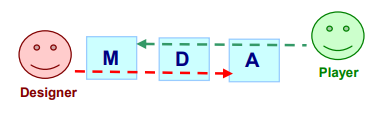
\includegraphics[height=0.48\textheight,keepaspectratio]{MDA.png}
\end{frame}

\begin{frame}{Octalysis}
  \centering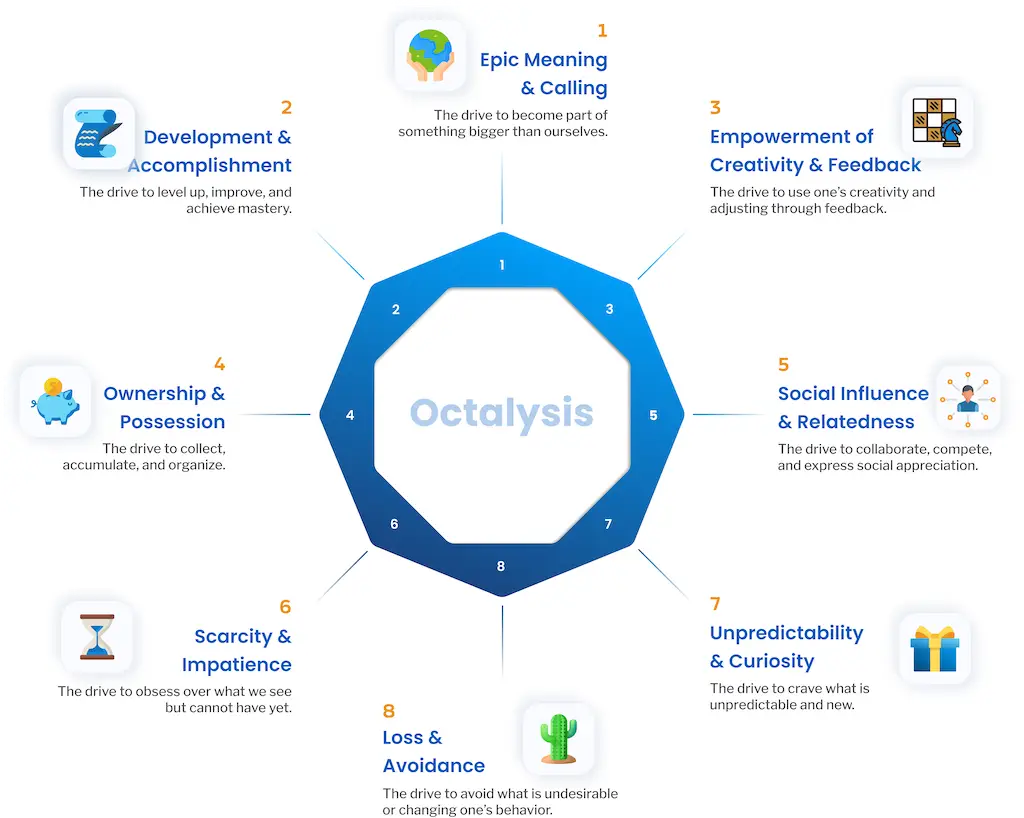
\includegraphics[height=0.9\textheight,keepaspectratio]{octalysis.jpg}
  \vfill
  \scriptsize\mbox{}\autocite{Chou2015}
\end{frame}

%==============================================================================
\begin{frame}{Welke elementen werken?}
  \footnotesize
  \begin{columns}[T]
    \begin{column}{0.56\textwidth}
      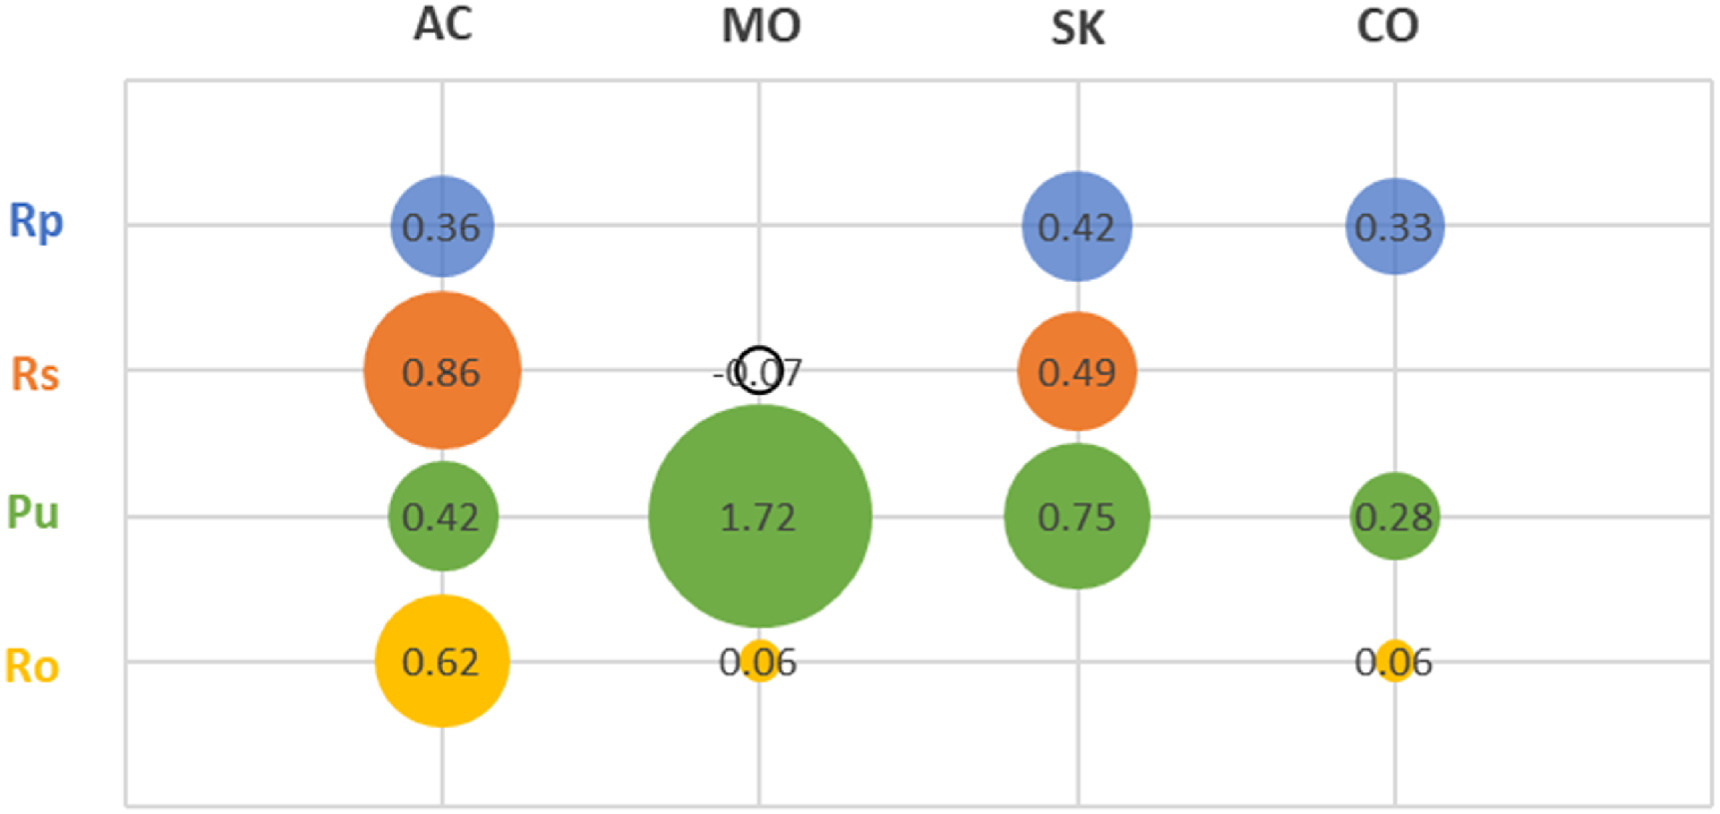
\includegraphics[height=0.42\textheight]{results_meta_analysis.jpg}
      \par\medskip
      \centering\scriptsize
      \setlength{\tabcolsep}{4pt}%
      \renewcommand{\arraystretch}{1.1}%
      \begin{tabular}{@{}l@{\hspace{1.2em}}l@{\hspace{1.8em}}l@{\hspace{1.2em}}l@{}}
        \multicolumn{4}{c}{\textbf{Legende}} \\[0.2em]
        \textbf{Rp} & prestatiebeloningen & \textbf{AC} & academische prestaties \\
        \textbf{Rs} & sociale beloningen & \textbf{MO} & motivatie \\
        \textbf{Pu} & puzzels/uitdagingen & \textbf{SK} & denkvaardigheden \\
        \textbf{Ro} & rollenspel & \textbf{CO} & cognitieve belasting \\
      \end{tabular}
    \end{column}
    \begin{column}{0.44\textwidth}
      Meta-analyse van Zhan et al.:
      \begin{itemize}
        \item Geaggregeerd (SMD): \(\approx 0{,}77\) op motivatie
        \item Geaggregeerd (SMD): \(\approx 0{,}75\) op prestaties
        \item Puzzels/Challenges (Pu): sterkst op motivatie (\(g \approx 1{,}72\))
        \item Rollenspel (Ro): verwaarloosbaar (\(g \approx 0{,}06\))
      \end{itemize}
      \medskip
      \scriptsize SMD = totale meta-analyse; \(g\) = Hedges' \(g\) per elementcategorie.
    \end{column}
  \end{columns}
  \vfill
  \scriptsize\mbox{}\autocite{Zhan2022}
\end{frame}

%==============================================================================
\section*{Proof-of-Concept}

\begin{frame}{Proof-of-Concept}
  \centering
  {\large\textcolor{hgblue}{\href{https://bap-cobol-gamification.vercel.app/}{bap-cobol-gamification.vercel.app}}}
  \vfill
\end{frame}

%==============================================================================
\section{Evaluatie en resultaten}

\begin{frame}{Evaluatie in twee delen}
  \begin{columns}[T]
    \begin{column}{0.5\textwidth}
      \begin{block}{Deel 1: literatuurevaluatie (uitgevoerd)}
        \footnotesize Elke ontwerpkeuze wordt afgezet tegen empirisch onderzoek. Per keuze: beschrijven, een claim uit de literatuur zoeken en beoordelen.
      \end{block}
    \end{column}
    \begin{column}{0.5\textwidth}
      \begin{block}{Deel 2: pilotontwerp (niet uitgevoerd)}
        \footnotesize Een reproduceerbaar experiment: twee groepen leren elk een dag COBOL, een via de PoC en een via een papieren cursus, gevolgd door dezelfde kennistest.
      \end{block}
    \end{column}
  \end{columns}
\end{frame}

%==============================================================================
\begin{frame}{Resultaten literatuurevaluatie}
  \footnotesize
  \begin{columns}[T]
    \begin{column}{0.4\textwidth}
      \textbf{Ontwerpkeuzes en literatuur}
      \begin{itemize}
        \item \textbf{PBL} \autocite{KevinWerbach2020}
        \item \textbf{Octalysis} \autocite{Chou2015}
      \end{itemize}
    \end{column}
    \begin{column}{0.6\textwidth}
      \centering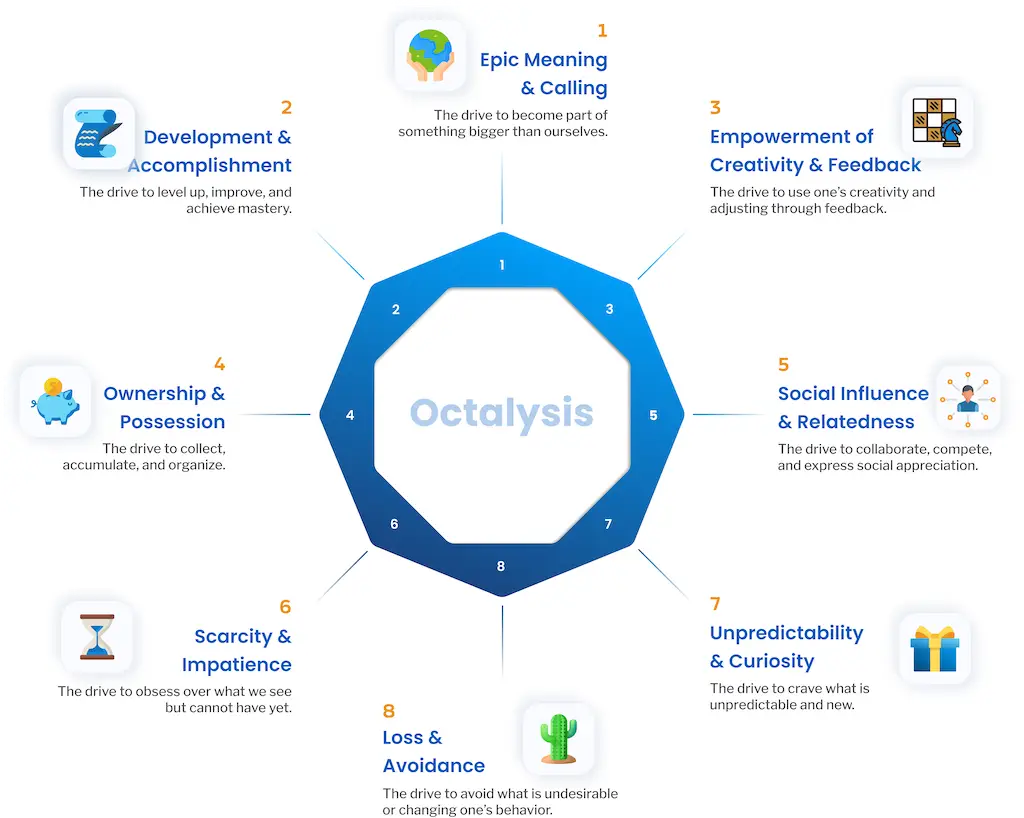
\includegraphics[width=0.9\textheight,keepaspectratio]{octalysis.jpg}
    \end{column}
  \end{columns}
\end{frame}

\begin{frame}{Verwacht effect op basis van literatuur}
  \footnotesize
  De PoC implementeert kerncomponenten uit de meta-analyse van Zhan et al.
  Effecten in vergelijkbare grootteorde zijn aannemelijk:
  \medskip
  \centering
  \begin{tikzpicture}[scale=0.78, transform shape]
    \node (e1) {\statcard{hgdarkgreen}{0{,}77}{motivatie (SMD)}{}};
    \node[right=0.32cm of e1] (e2) {\statcard{hgblue}{0{,}75}{prestaties (SMD)}{}};
    \node[right=0.32cm of e2] (e3) {\statcard{hgorange}{1{,}72}{challenges/puzzels op motivatie (\(g\))}{}};
    \node[right=0.32cm of e3] (e4) {\statcard{hgpurple}{0{,}06}{rollenspel op motivatie (\(g\))}{}};
  \end{tikzpicture}
  \vfill
  \scriptsize
  SMD = geaggregeerde meta-analyse;\\
  \(g\) = Hedges' \(g\) per elementcategorie.\autocite{Zhan2022}
\end{frame}

%==============================================================================
\begin{frame}{Beperkingen}
  \begin{itemize}
    \item \textbf{Geen empirische geldigheid voor de PoC zelf}
    \item \textbf{Selectiebias:} de meta-analyses gaan vooral over moderne talen, niet over COBOL.
    \item \textbf{Confounding:} een deel van het effect komt door interactiviteit op zich, niet enkel door gamification \autocite{Zhan2022}.
    \item \textbf{Heuristische validatie:} regex-checks kunnen false positives en false negatives geven.
  \end{itemize}
\end{frame}

%==============================================================================
\begin{frame}
  \centering
  \vfill
  {\Huge\textbf{Bedankt}}\\[14pt]
  {\Large Vragen?}\\[20pt]
  \footnotesize Silas De Vuyst \quad\textbar\quad
  \textcolor{hgblue}{\href{https://bap-cobol-gamification.vercel.app/}{bap-cobol-gamification.vercel.app}}
  \vfill
\end{frame}

%==============================================================================
\begin{frame}[allowframebreaks]{Referenties}
  \printbibliography[heading=none]
\end{frame}

\end{document}
